\section{分析結果}

\subsection{不同語音離散表徵的比較}

{


\begin{table}[!htbp]
    \centering
    \begin{subtable}[t]{\textwidth}
        \centering
        \begin{tabular}{|c|c|c|c|c|c|} \hline
                        & 音位純度   & 分群純度   & 音位熵    & 離散單元熵  & PNMI   \\ \hline
            HuBERT      &     0.5256 &     0.3382 &    3.3152 &      3.8681 & 0.4993 \\ \hline    %% 1.6552 h
            Wav2vec 2.0 &     0.4006 &     0.2676 &    3.3152 &      3.8215 & 0.3706 \\ \hline    %% 1.2286 w
            CPC         &     0.5188 &     0.3812 &    3.3146 &      3.7918 & 0.4992 \\ \hline    %% 1.6545 c
            LogMel      &     0.3253 &     0.1473 &    3.3158 &      3.8630 & 0.2647 \\ \hline    %% 0.8776 l 
        \end{tabular}
        \caption{群數 = 50}
        \label{tab:ch3-clu050-phn}
    \end{subtable}

    \vspace{0.5cm}

    \begin{subtable}[t]{\textwidth}
        \centering
        \begin{tabular}{|c|c|c|c|c|c|} \hline
                        & 音位純度   & 分群純度   & 音位熵    & 離散單元熵  & PNMI   \\ \hline
            HuBERT      &     0.6097 &     0.2553 &    3.3152 &      4.5704 & 0.5786 \\ \hline    %% 1.9181 h
            Wav2vec 2.0 &     0.4877 &     0.2118 &    3.3152 &      4.5284 & 0.4596 \\ \hline    %% 1.5235 w
            CPC         &     0.5895 &     0.2674 &    3.3146 &      4.5034 & 0.5557 \\ \hline    %% 1.8418 c
            LogMel      &     0.3348 &     0.0931 &    3.3158 &      4.5591 & 0.2789 \\ \hline    %% 0.9247 l 
        \end{tabular}
        \caption{群數 = 100}
        \label{tab:ch3-clu100-phn}
    \end{subtable}

    \vspace{0.5cm}

    \begin{subtable}[t]{\textwidth}
        \centering
        \begin{tabular}{|c|c|c|c|c|c|} \hline
                        & 音位純度   & 分群純度   & 音位熵    & 離散單元熵  & PNMI   \\ \hline
            HuBERT      &     0.6474 &     0.1644 &    3.3152 &      5.2681 & 0.6289 \\ \hline    %% 2.0849 h
            Wav2vec 2.0 &     0.5427 &     0.1467 &    3.3152 &      5.2173 & 0.5188 \\ \hline    %% 1.7199 w
            CPC         &     0.6098 &     0.1789 &    3.3146 &      5.1885 & 0.5882 \\ \hline    %% 1.9497 c
            LogMel      &     0.3474 &     0.0569 &    3.3158 &      5.2322 & 0.2955 \\ \hline    %% 0.9798 l 
        \end{tabular}
        \caption{群數 = 200}
        \label{tab:ch3-clu200-phn}
    \end{subtable}

    \caption{不同群數在四種基石模型的音位分析數據}
    \label{tab:single-cluster-results}
\end{table}

}

{
\begin{figure}
     \centering
     \begin{subfigure}[t]{0.3\textwidth}
         \centering
         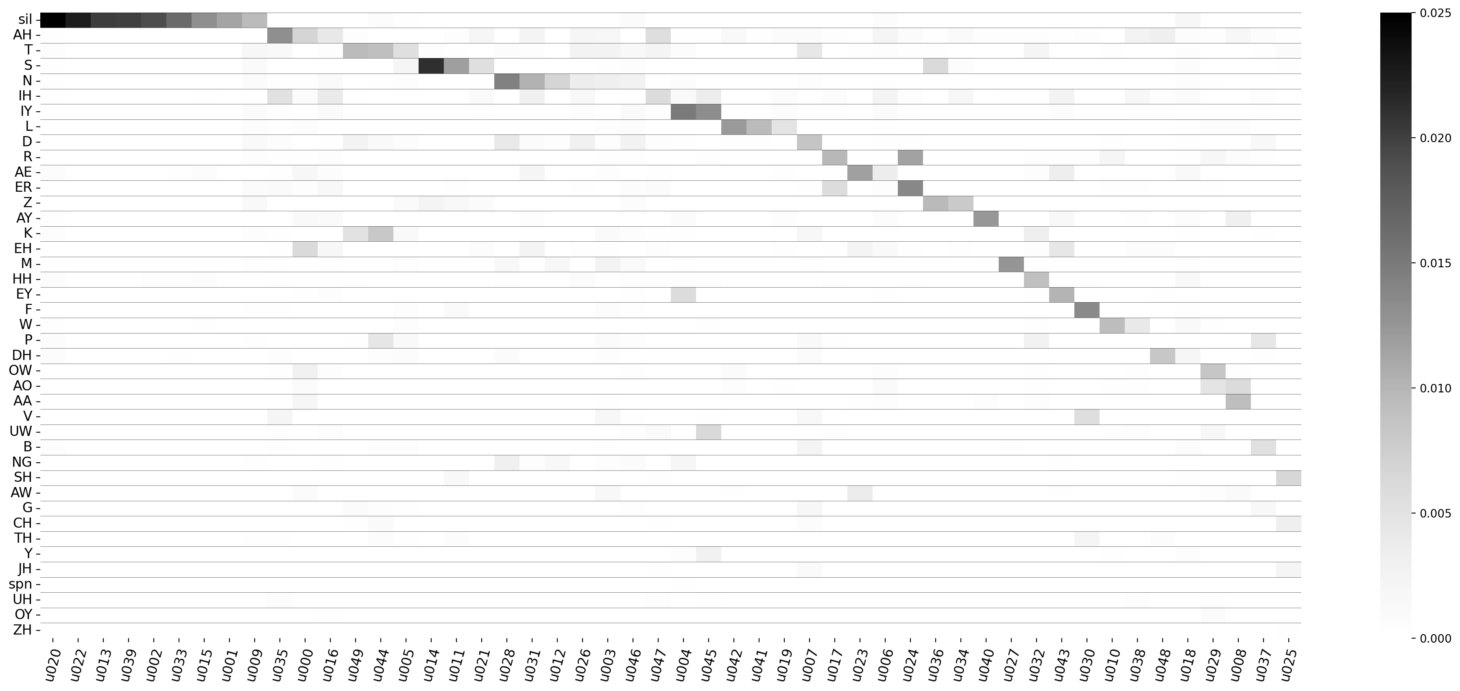
\includegraphics[width=1\linewidth]{figures/hubert-50-joint-byprob--new1.png}
         \caption{hubert}
         \label{fig:ch3-heatmap-model--hubert-50-joint-byprob}
     \end{subfigure}
     \vfill
     \begin{subfigure}[t]{0.3\textwidth}
         \centering
         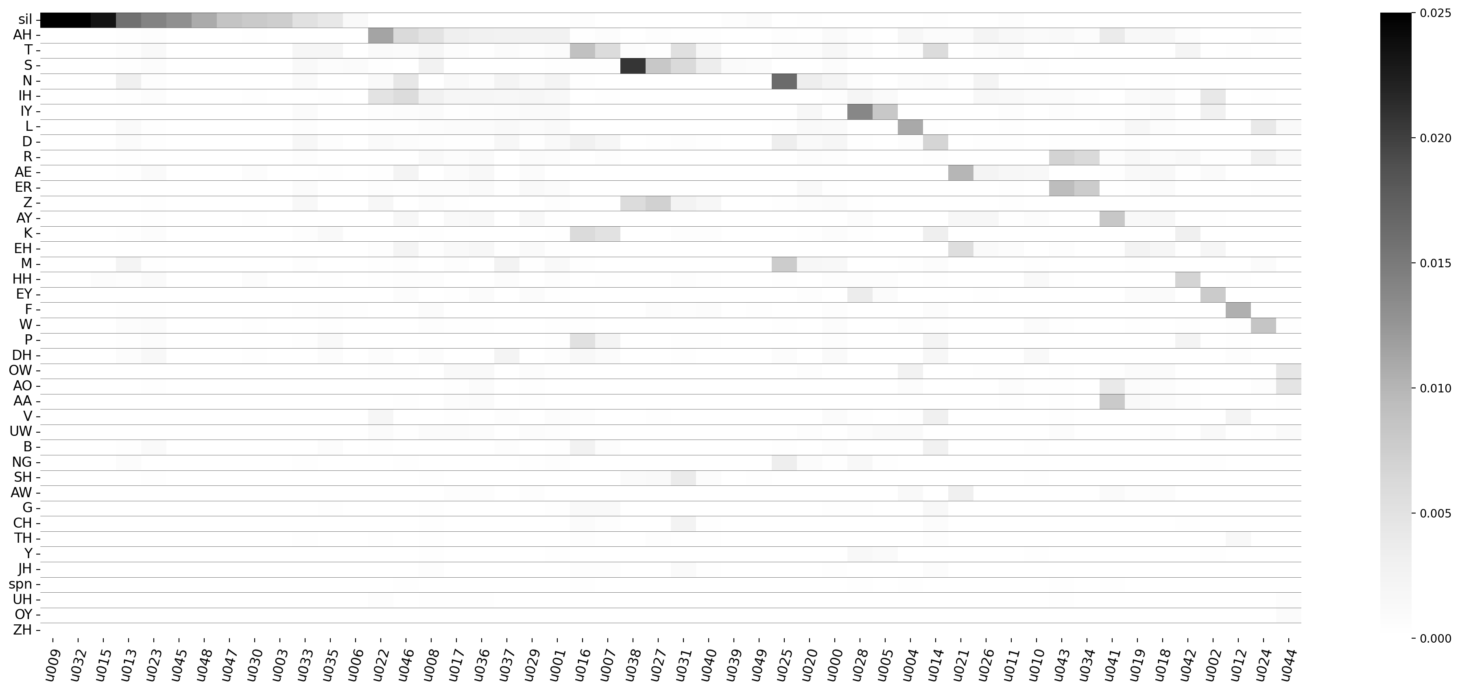
\includegraphics[width=1\linewidth]{figures/w2v2-50-joint-byprob.png}
         \caption{w2v2}
         \label{fig:ch3-heatmap-model--w2v2-50-joint-byprob}
     \end{subfigure}
     \vfill
     \begin{subfigure}[t]{0.3\textwidth}
         \centering
         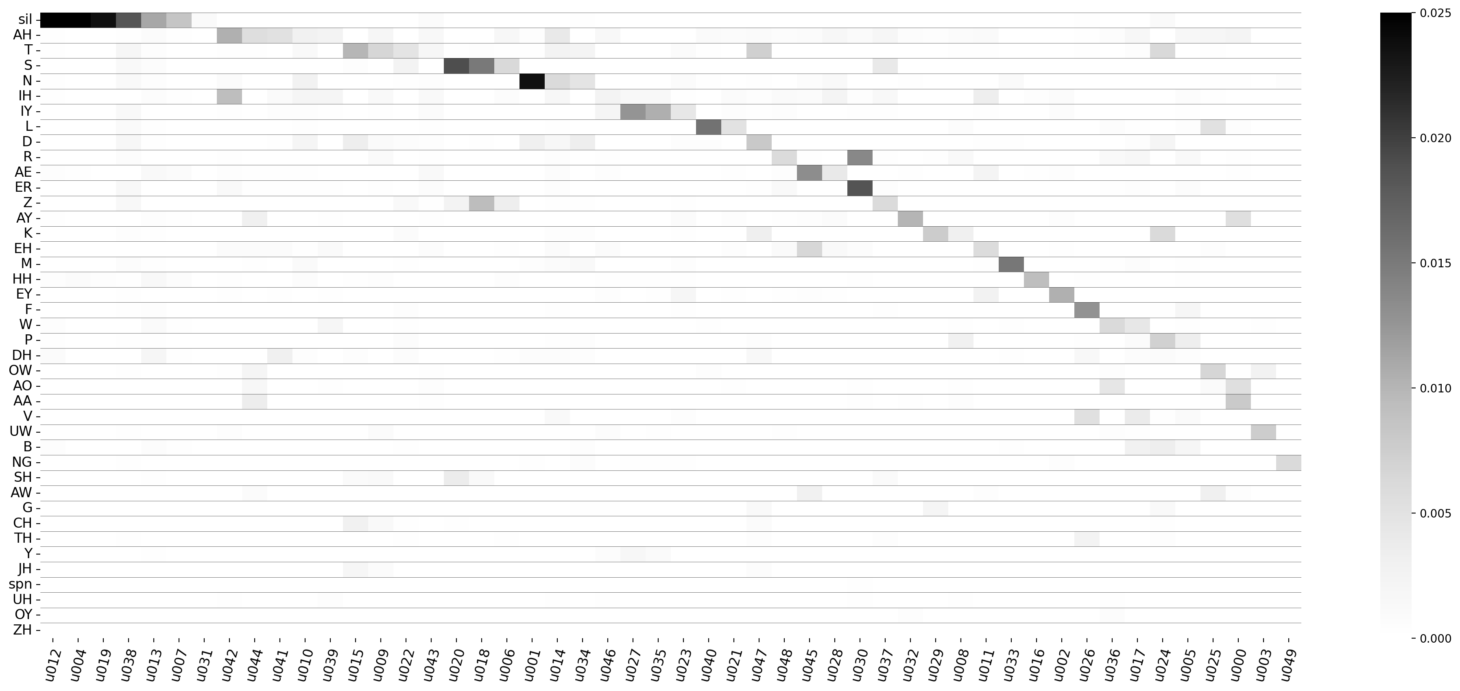
\includegraphics[width=1\linewidth]{figures/cpc-50-joint-byprob.png}
         \caption{cpc}
         \label{fig:ch3-heatmap-model--cpc-50-joint-byprob}
     \end{subfigure}
     \vfill
     \begin{subfigure}[t]{0.3\textwidth}
         \centering
         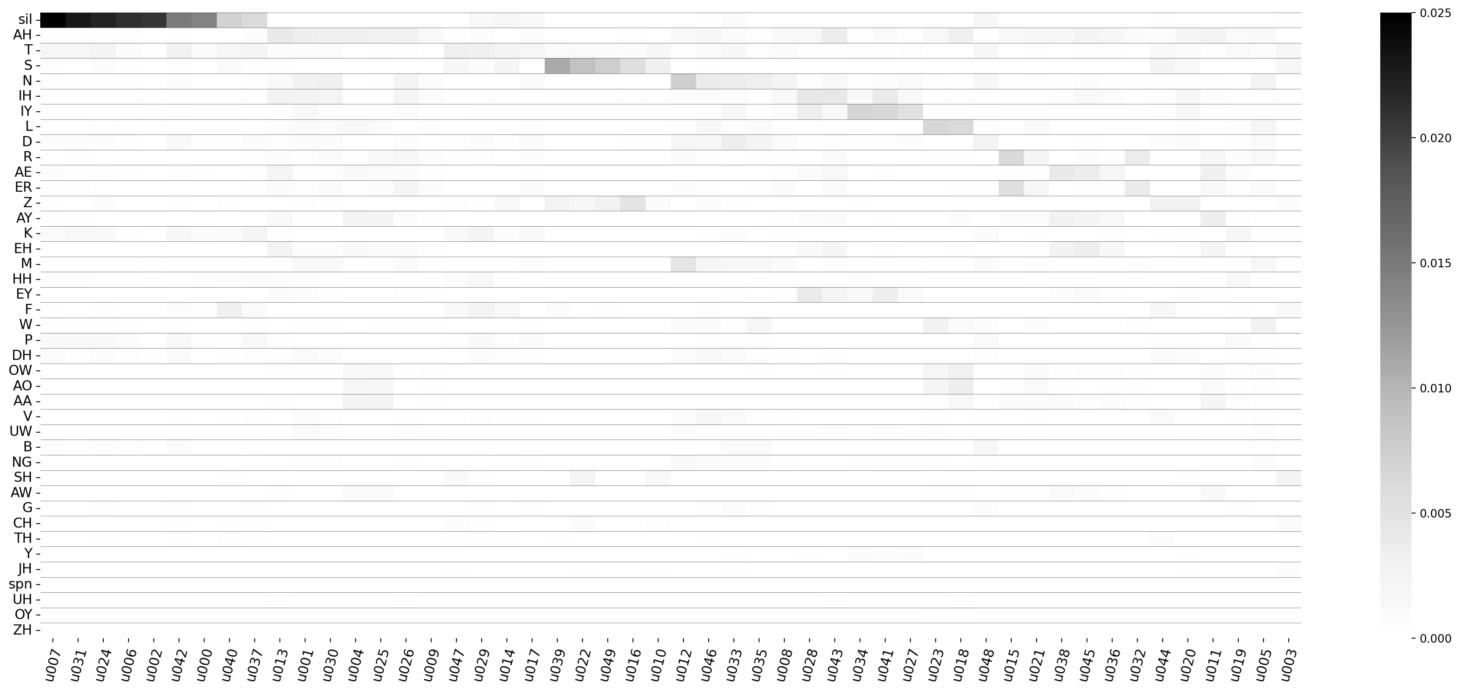
\includegraphics[width=1\linewidth]{figures/logmel-50-joint-byprob.png}
         \caption{logmel}
         \label{fig:ch3-heatmap-model--logmel-50-joint-byprob}
     \end{subfigure}
     \caption{模型比較}
     \label{fig:ch3-heatmap-model-comparison}
\end{figure}
}
  
          首先,表 \ref{tab:single-cluster-results} 比較了不同模型的純度與相互資訊的數據,而這四個離散表徵的機率分佈圖於 \ref{fig:ch3-heatmap-model-comparison} 中呈現。從這些分析結果,我們可以觀察到 HuBERT 和 CPC 對於捕捉音素之間的關係是比較好的,音位純度與分群純度都較高這點,也在熱圖上以較為清晰深色的格子呈現。由此可以說明 HuBERT 和 CPC 模型在捕捉訊號中的發音特徵能力效果較 Wav2vec 2.0 和聲學特徵的 LogMel 好上不少。同樣的趨勢在群數為 100 和 200 時也能被觀察出來,尤其又以 HuBERT 效果明顯好上不少。

        除了從熱圖與純度觀察,我們也可以觀察每個模型對應離散單元所對應的音素的條件音素熵分佈,來探討這些離散單元捕捉音素分佈的效果。圖 \ref{fig:ch3-heatmap-model-comparison} 展示了四種模型的音素熵分佈直方圖,比較四個模型在群數 50 和 100 的直方圖,我們也可以得到和前段相同的結論 --- HuBERT 的表現是四個模型中最好的。

        因此,我們可以著重觀察 HuBERT,進一步比較三個不同分群數的機率熱圖。依循 hao sptok dinosr 等,我們在這邊以條件機率呈現。從圖中可以發現,當分群數量上升時,離散單元之間有對區分不同音素的效果得到提升,\cite{10.5555/177910.177914}。